% EQTC 2026 poster -- A0 portrait (841 x 1189 mm), layout after "EQTC 2026 - Poster Template.pdf":
% centred title block, two columns, sources + contact footer.
% Compiles with pdfLaTeX on Overleaf. Upload this file, table_results.tex and figures/.
% Figures and the table are generated by make_poster_figures.py (run from the repo root).
\documentclass{article}
\usepackage[paperwidth=841mm,paperheight=1189mm,margin=30mm]{geometry}
\usepackage[T1]{fontenc}
\usepackage[utf8]{inputenc}
\usepackage{tgheros}                 % Helvetica clone; the template uses Arial
\renewcommand{\familydefault}{\sfdefault}
\usepackage{amsmath}
\usepackage[helvet]{sfmath}          % sans-serif math to match the text
\usepackage{anyfontsize}
\usepackage{graphicx}
\usepackage{xcolor}
\usepackage{booktabs}
\usepackage{caption}
\usepackage{enumitem}
\usepackage{tikz}
\usetikzlibrary{arrows.meta,calc,positioning}

\definecolor{ink}{HTML}{0B0B0B}
\definecolor{muted}{HTML}{52514E}
\definecolor{rulegray}{HTML}{E4E3DF}
\definecolor{qblue}{HTML}{2A78D6}
\definecolor{qbluelight}{HTML}{86B6EF}
\definecolor{qbluefill}{HTML}{CDE2FB}
\definecolor{qgray}{HTML}{8A8983}

\pagestyle{empty}
\setlength{\parindent}{0pt}
\setlength{\parskip}{0pt}
\color{ink}

% ---- type scale (A0: body ~28 pt) -------------------------------------------------
\newcommand{\bodyfont}{\fontsize{28}{37}\selectfont}
\newcommand{\smallfont}{\fontsize{23}{29}\selectfont}
\newcommand{\tinyfont}{\fontsize{19}{24}\selectfont}

\newcommand{\psection}[1]{%
  {\fontsize{46}{54}\selectfont\bfseries #1\par}
  \vspace{5mm}{\color{qblue}\rule{90mm}{2.5mm}}\par\vspace{9mm}}

\DeclareCaptionFont{postercap}{\smallfont\color{muted}}
\captionsetup{font=postercap,labelfont=bf,skip=6mm,justification=justified,singlelinecheck=false}

\setlist[itemize]{leftmargin=11mm,itemsep=5mm,topsep=3mm,parsep=0pt,
  label={\color{qblue}\rule[0.25ex]{0.55em}{0.55em}}}

\newlength{\colw}\setlength{\colw}{\dimexpr(\textwidth-34mm)/2\relax}
\newlength{\bodyh}\setlength{\bodyh}{850mm}

\tikzset{
  every node/.style={font=\smallfont},
  box/.style={draw=qblue,line width=2pt,fill=qbluefill,rounded corners=4mm,
              align=center,text width=#1,inner sep=5mm,minimum height=48mm},
  box/.default=70mm,
  flow/.style={-{Latex[length=7mm,width=6mm]},line width=3pt,draw=ink},
  panel/.style={font=\fontsize{26}{32}\selectfont\bfseries,anchor=north west},
}

\begin{document}
\bodyfont

% ==================================================================================
% Title block
% ==================================================================================
\begin{center}
  {\fontsize{64}{77}\selectfont\bfseries
   A Hybrid Quantum-Inspired Evolutionary Algorithm with Adaptive\\
   Rotation-Gate Control for Many-Objective Vehicle Routing\par}
  \vspace{12mm}
  {\fontsize{50}{60}\selectfont Diagnosis, Correction, and Comparative Evaluation\par}
  \vspace{14mm}
  {\fontsize{38}{46}\selectfont Olivian-Antonio G\^{\i}lea, Adrian Florea, Claudia Banciu\par}
  \vspace{6mm}
  {\fontsize{30}{38}\selectfont\color{muted} Computer Science and Electrical Engineering Department,
   ``Lucian Blaga'' University of Sibiu, Romania\par}
\end{center}
\vspace{10mm}
{\color{rulegray}\rule{\textwidth}{2mm}}
\vspace{16mm}

% ==================================================================================
% Left column
% ==================================================================================
\noindent
\begin{minipage}[t][\bodyh][t]{\colw}

\psection{Motivation}
\begin{itemize}
  \item Quantum-inspired evolutionary algorithms (QIEAs) encode each gene as a qubit angle
        and search with rotation gates. Recent quantum and quantum-inspired multi-objective
        work stays on synthetic or 2--3-objective problems [1,\,2].
  \item Our earlier multi-objective QIEA on Sibiu waste routing lost population diversity
        as instances grew, caused by its repair step for infeasible tours [3].
  \item \textbf{Question:} can a decomposition-guided QIEA match established
        many-objective evolutionary algorithms on a real \textbf{5-objective} routing problem?
\end{itemize}

\vfill
\psection{Method: HQIEA-ARGC}

\begin{center}
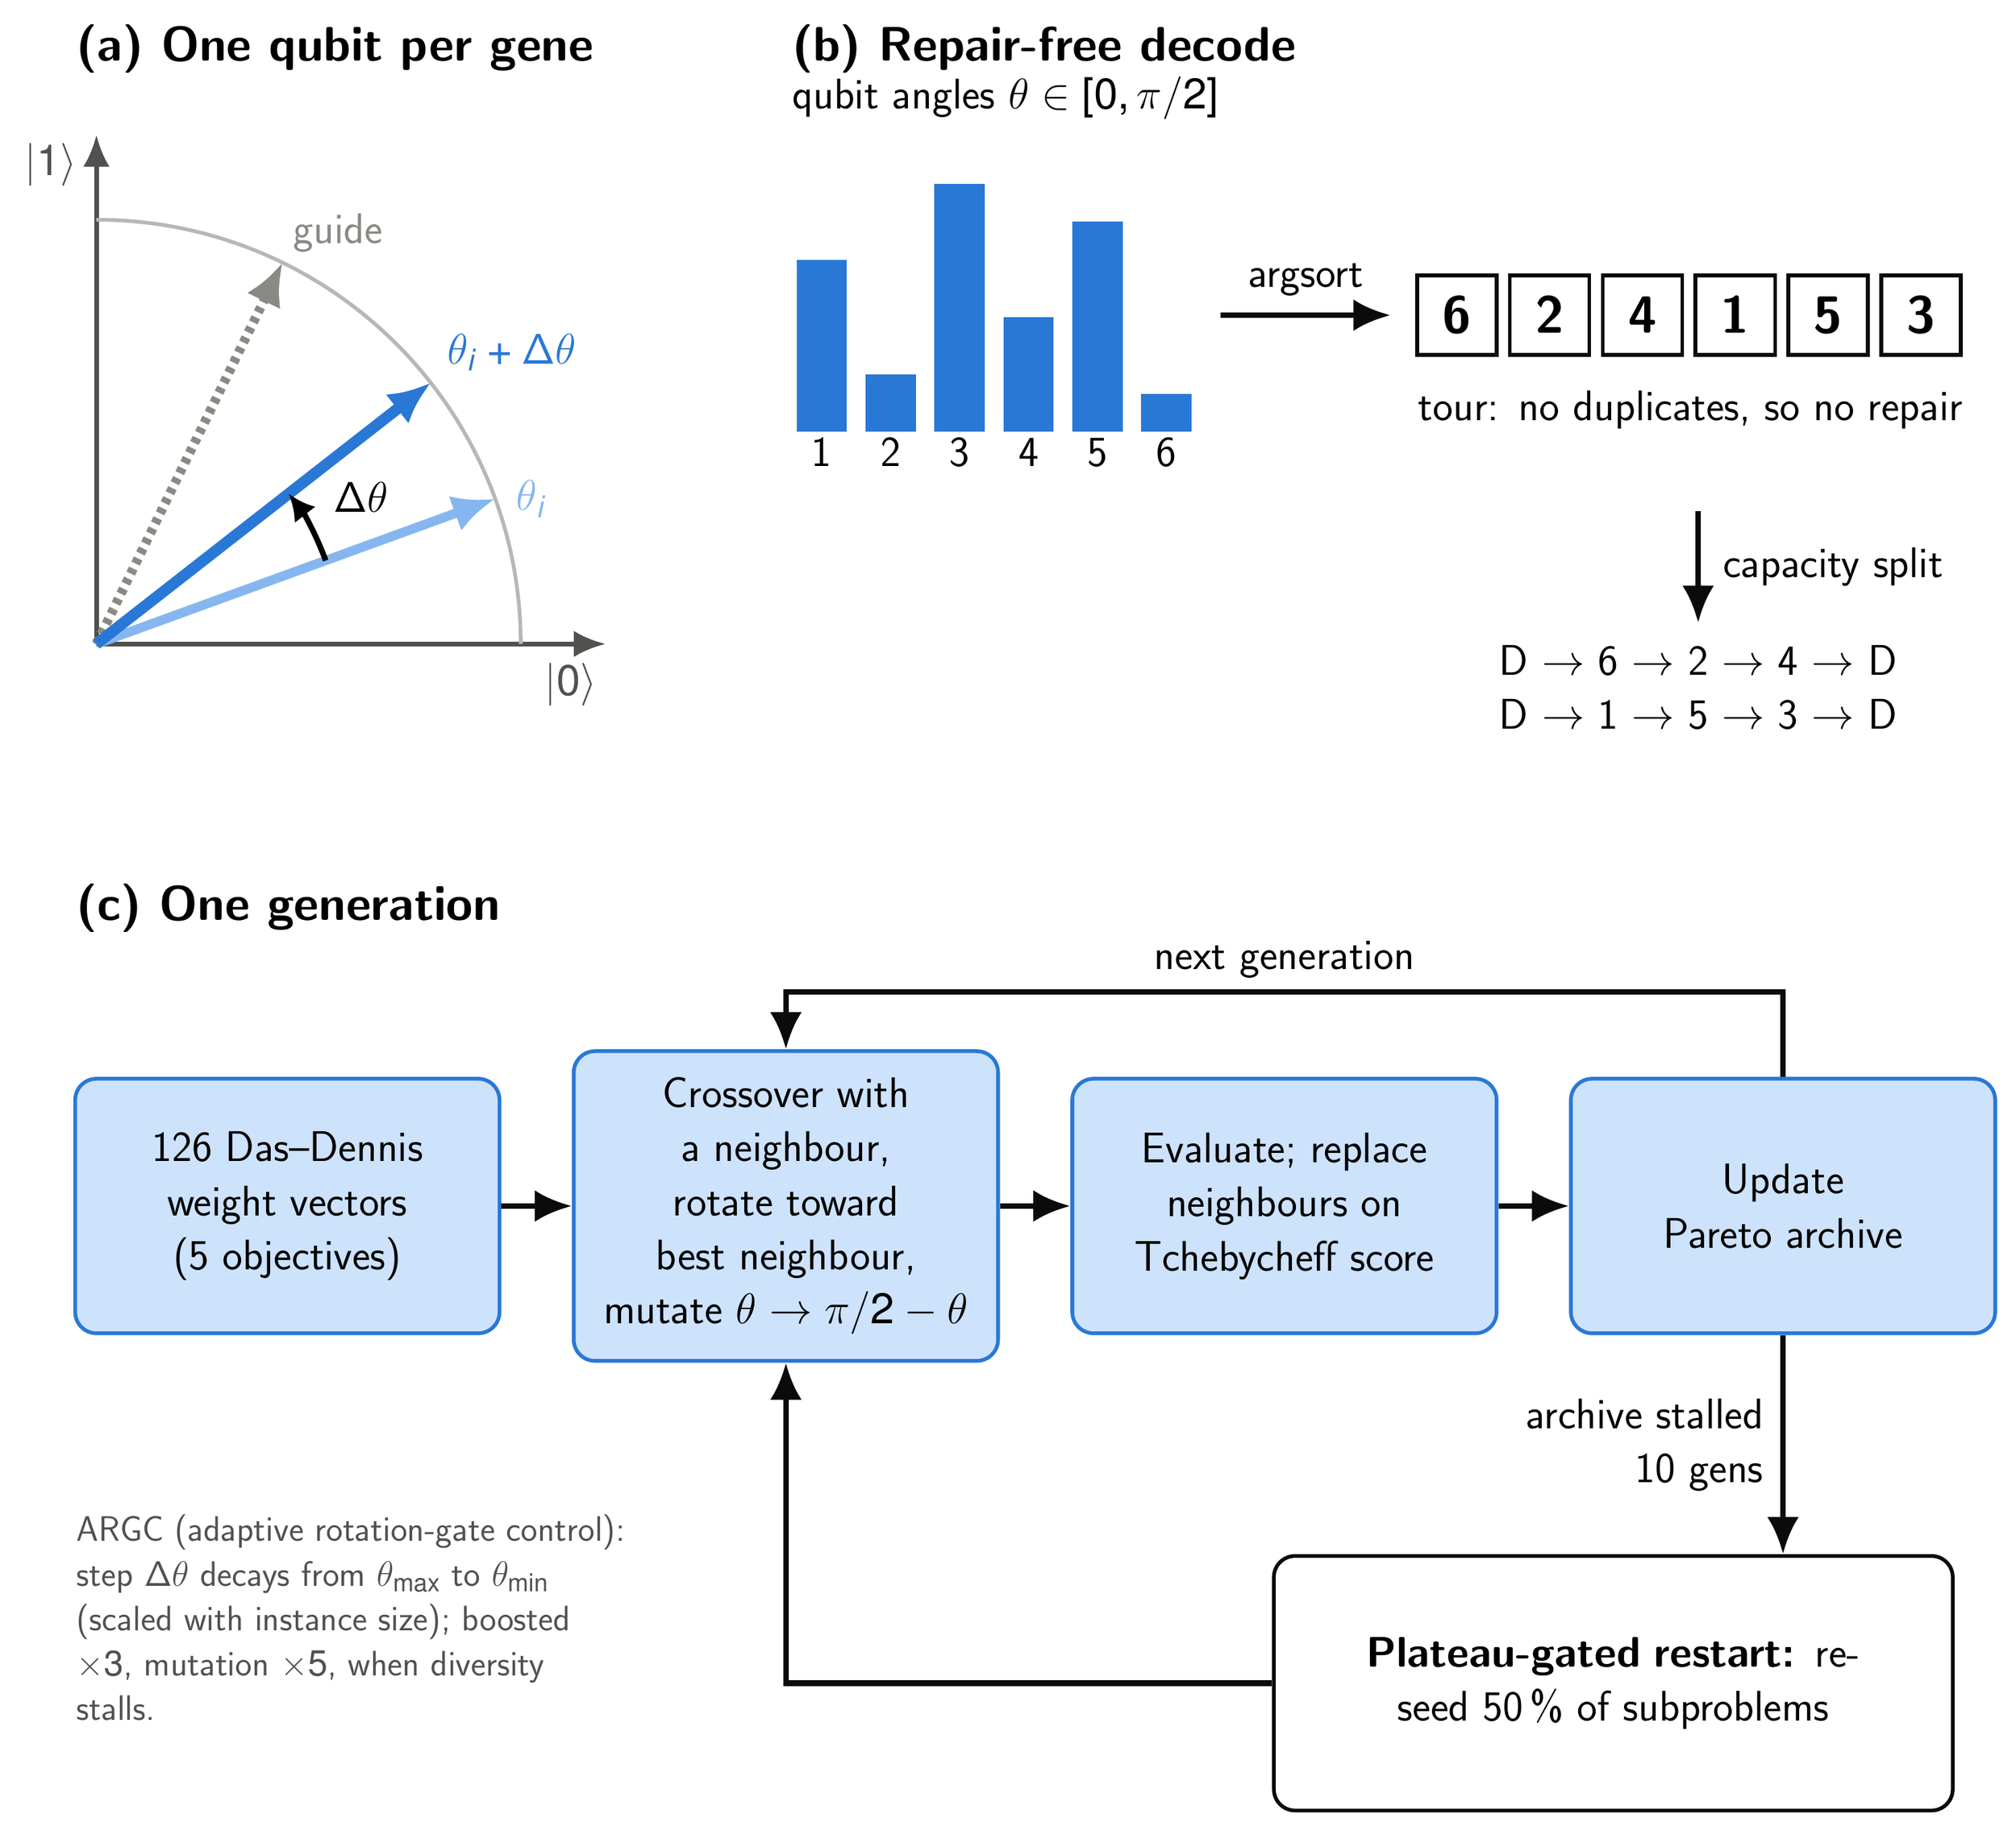
\begin{tikzpicture}[x=1cm,y=1cm]
  % ---------- (a) qubit gene ----------
  \node[panel] at (-0.5,11.8) {(a) One qubit per gene};
  \draw[-{Latex[length=6mm,width=5mm]},line width=2.5pt,muted] (0,0) -- (9.6,0)
        node[below left=2mm and 0mm] {$|0\rangle$};
  \draw[-{Latex[length=6mm,width=5mm]},line width=2.5pt,muted] (0,0) -- (0,9.6)
        node[below left=0mm and 2mm] {$|1\rangle$};
  \draw[line width=2pt,rulegray!70!muted] (8,0) arc (0:90:8);
  \draw[-{Latex[length=8mm,width=7mm]},line width=5pt,qgray,dashed] (0,0) -- (64:8)
        node[above right=0mm and 0mm] {guide};
  \draw[-{Latex[length=8mm,width=7mm]},line width=5pt,qbluelight] (0,0) -- (20:8)
        node[right=2mm] {$\theta_i$};
  \draw[-{Latex[length=8mm,width=7mm]},line width=6pt,qblue] (0,0) -- (38:8)
        node[above right=0mm and 1mm] {$\theta_i+\Delta\theta$};
  \draw[-{Latex[length=5mm,width=5mm]},line width=3pt] (20:4.6) arc (20:38:4.6);
  \node at (29:5.7) {$\Delta\theta$};

  % ---------- (b) repair-free decode ----------
  \node[panel] at (13,11.8) {(b) Repair-free decode};
  \foreach \ang/\lab [count=\i] in {0.9/1,0.3/2,1.3/3,0.6/4,1.1/5,0.2/6} {
    \pgfmathsetmacro{\x}{13.2+1.3*(\i-1)}
    \fill[qblue] (\x,4) rectangle ++(0.95,{3.6*\ang});
    \node[below] at ({\x+0.475},4) {\lab};
  }
  \node[anchor=west] at (13,10.3) {qubit angles $\theta \in [0,\pi/2]$};
  \draw[flow] (21.2,6.2) -- (24.4,6.2) node[midway,above=2mm] {argsort};
  \foreach \lab [count=\i] in {6,2,4,1,5,3} {
    \node[draw=ink,line width=2pt,minimum size=15mm,inner sep=0pt,fill=white,
          font=\bodyfont\bfseries] at ({24.9+1.75*(\i-1)+0.75},6.2) {\lab};
  }
  \node[anchor=north west,text width=10.5cm,align=left] at (24.8,4.9)
       {tour: no duplicates, so no repair};
  \draw[flow] (30.2,2.5) -- (30.2,0.4) node[midway,right=3mm] {capacity split};
  \node[anchor=north,align=left] at (30.2,0.1)
       {D $\to$ 6 $\to$ 2 $\to$ 4 $\to$ D\\ D $\to$ 1 $\to$ 5 $\to$ 3 $\to$ D};

  % ---------- (c) one generation ----------
  \node[panel] at (-0.5,-4.4) {(c) One generation};
  \node[box] (w)  at (3.6,-10.6)  {126 Das--Dennis\\weight vectors\\(5 objectives)};
  \node[box] (o)  at (13.0,-10.6) {Crossover with a neighbour, rotate toward best neighbour,
                                    mutate $\theta\to\pi/2-\theta$};
  \node[box] (e)  at (22.4,-10.6) {Evaluate; replace neighbours on Tchebycheff score};
  \node[box] (a)  at (31.8,-10.6) {Update Pareto archive};
  \draw[flow] (w) -- (o);
  \draw[flow] (o) -- (e);
  \draw[flow] (e) -- (a);
  \draw[flow] (a.north) -- ++(0,1.6) -| node[pos=0.25,above=1mm] {next generation} (o.north);
  \node[box=118mm,draw=ink,fill=white] (r) at (28.6,-19.6)
       {\textbf{Plateau-gated restart:} reseed 50\,\% of subproblems};
  \draw[flow] (a.south) -- node[left=2mm,align=right] {archive stalled\\10 gens} (a.south |- r.north);
  \draw[flow] (r.west) -| (o.south);
  \node[anchor=north west,text width=10.5cm,align=left,font=\tinyfont,text=muted]
       at (-0.5,-16.3)
       {ARGC (adaptive rotation-gate control): step $\Delta\theta$ decays from
        $\theta_{\max}$ to $\theta_{\min}$ (scaled with instance size); boosted $\times3$,
        mutation $\times5$, when diversity stalls.};
\end{tikzpicture}
\end{center}

\vspace{2mm}
{\smallfont\color{muted} MOEA/D-style decomposition: one individual per Tchebycheff
subproblem, mating within the 10 nearest subproblems.\par}

\vfill
\psection{Problem and protocol}
Sibiu waste collection as a capacitated vehicle routing problem (CVRP) with
\textbf{five minimised objectives}: distance, travel time (congestion factor per edge),
cost (fixed per vehicle + fuel),
CO$_2$ (payload grows along each route) and workload balance (std.\ of route times).
A capacity-first split makes every solution feasible.
\begin{itemize}
  \item \textbf{7 instances:} 4 CVRPLIB (32--200 nodes) and 3 Sibiu routes with real
        distances (199--334 nodes). Demand, capacity, congestion and cost/emission
        coefficients are synthesised (fixed seed).
  \item \textbf{Baselines:} NSGA-II, SPEA2, MOEA/D, RVEA (pymoo [4]); MOEA/D, RVEA and
        HQIEA-ARGC share 126 weight vectors, NSGA-II/SPEA2 use a population of 80.
  \item \textbf{Protocol:} 30 runs $\times$ 500 generations per instance; hypervolume (HV)
        against a shared reference point; Wilcoxon and Friedman tests.
\end{itemize}

\end{minipage}%
\hfill
% ==================================================================================
% Right column
% ==================================================================================
\begin{minipage}[t][\bodyh][t]{\colw}

\psection{Diagnosis: the population froze}
In the first full-scale campaign HQIEA-ARGC was last on all 7 instances (0.17--0.45 of
the best baseline's HV). Its HV froze early, and the ARGC boost almost never fired, so
once the subproblems converged nothing renewed the search.

\vspace{6mm}
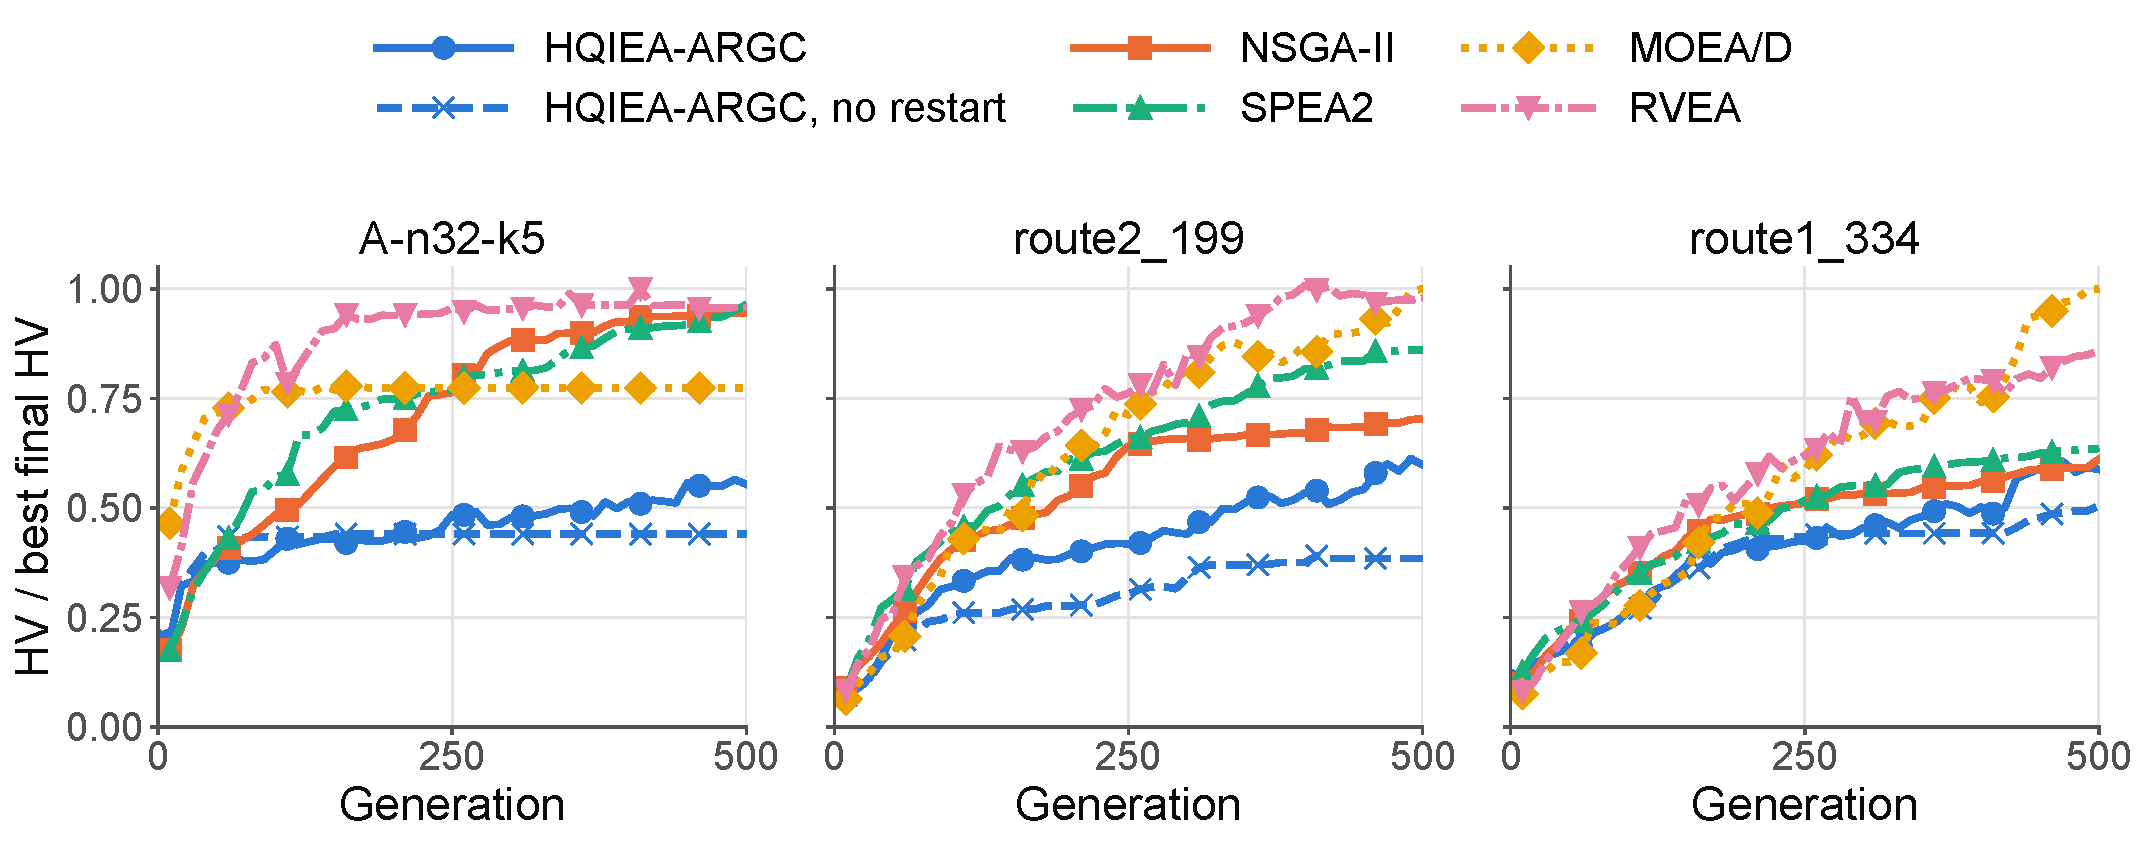
\includegraphics[width=\linewidth]{figures/trace.pdf}
\captionof{figure}{HV per generation, normalised to the best final HV (median of 3 seeds).
Without restart (dashed) HQIEA-ARGC stalls (A-n32-k5: from about generation 60) while
most baselines keep climbing.}

\vfill
\psection{Correction: plateau-gated restart}
When the archive stops growing for 10 generations, half of the subproblems get random
new angles; the rest are kept. HV rose \textbf{+27.7\,\% to +66.0\,\% on all
7 instances} ($p<0.005$ each), the most consistent gain in our study.

\vspace{6mm}
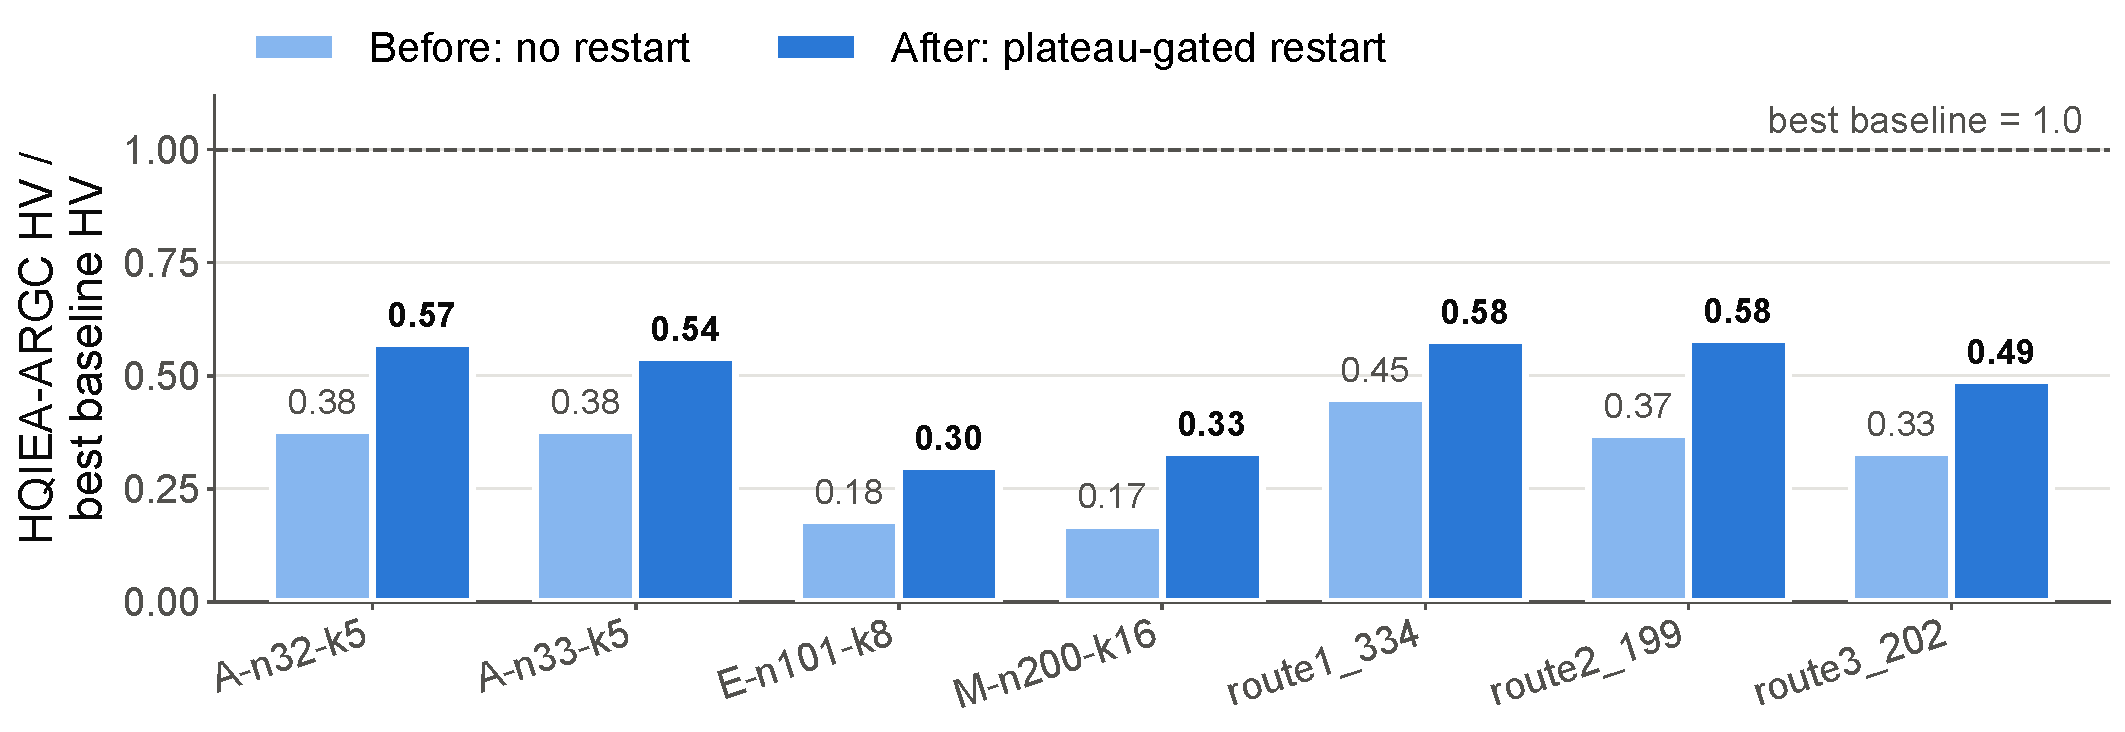
\includegraphics[width=\linewidth]{figures/restart_ratio.pdf}
\captionof{figure}{Mean HV relative to the best baseline (30 runs $\times$ 500 generations).}

\vfill
\psection{Comparison with baselines}
HQIEA-ARGC is still last everywhere; its one tie is with NSGA-II on route1\_334.

\vspace{6mm}
{\smallfont
\setlength{\tabcolsep}{3mm}
\begin{tabular*}{\linewidth}{@{}l@{\extracolsep{\fill}}rrrrrr@{}}
\toprule
\textbf{Instance} & \textbf{Restart gain} & \textbf{NSGA-II} & \textbf{SPEA2} &
\textbf{MOEA/D} & \textbf{RVEA} & \textbf{HQIEA-ARGC} \\
\midrule
% generated by make_poster_figures.py -- do not edit by hand
A-n32-k5 & +29.7\% & 0.99 & 0.99 & 0.88 & \textbf{1.00} & 0.57 \\
A-n33-k5 & +32.0\% & 0.96 & \textbf{1.00} & 0.84 & 0.99 & 0.54 \\
E-n101-k8 & +66.0\% & 0.48 & 0.54 & 0.98 & \textbf{1.00} & 0.30 \\
M-n200-k16 & +35.4\% & 0.37 & 0.43 & \textbf{1.00} & 0.93 & 0.33 \\
route1\_334 & +27.7\% & 0.61$^{\approx}$ & 0.69 & \textbf{1.00} & 0.93 & 0.58 \\
route2\_199 & +36.1\% & 0.75 & 0.81 & 0.99 & \textbf{1.00} & 0.58 \\
route3\_202 & +40.4\% & 0.66 & 0.72 & 0.90 & \textbf{1.00} & 0.49 \\

\bottomrule
\end{tabular*}\par}
\captionof{table}{Mean HV relative to the best algorithm (bold). Restart gain: with vs.\
without restart, 20 paired seeds, $p<0.005$ each. $\approx$: tied with HQIEA-ARGC
($p=0.24$); all other baselines significantly better ($p\le0.002$). Friedman
$p<10^{-14}$ on every instance.}

\vfill
\psection{Take-home messages}
\begin{itemize}
  \item \textbf{Repair-free:} argsort decoding gives valid tours on 5-objective
        routing up to 334 nodes, with no repair or penalty terms.
  \item \textbf{Diagnose before tuning:} a per-generation trace found the failure that
        parameter tuning had missed.
  \item \textbf{A gap remains} (0.30--0.58 of the best HV). Step size, mutation rate,
        neighbourhood and population size are ruled out as causes. Next: reference-vector
        selection, as in RVEA and MOEA/D.
\end{itemize}

\end{minipage}

% ==================================================================================
% Footer: sources and contact
% ==================================================================================
\vfill
{\color{rulegray}\rule{\textwidth}{2mm}}\par
\vspace{8mm}
\noindent
\begin{minipage}[t]{0.72\textwidth}
\tinyfont
[1] A.~Kotil et al., Quantum approximate multi-objective optimization, arXiv:2503.22797 (2025).\par
[2] A.~D.~King, Multi-objective optimization by quantum annealing, arXiv:2511.01762 (2025).\par
[3] O.-A.~G\^{\i}lea, A.~Florea, C.~Banciu, A.~Telcean, Scalable quantum-inspired evolutionary
algorithm for multi-objective optimization: real-world problems, manuscript in preparation (2026).\par
[4] J.~Blank, K.~Deb, pymoo: Multi-objective optimization in Python, IEEE Access 8,
89497--89509 (2020).
\end{minipage}%
\hfill
\begin{minipage}[t]{0.25\textwidth}
\raggedleft\tinyfont
\copyright\ 2026 the authors\\
Contact: olivianantonio.gilea@ulbsibiu.ro
\end{minipage}

\end{document}
